\section{Thorin measures along vertical lines}\label{bsy:sec:thorin}

Write $\rho=\beta+i\gamma$ for the zeros of $\zeta$ (the zeros of $\xi$), counted with multiplicity. For $\sigma>\frac12$ that is not the real part of a zero let $\mathfrak U_\sigma$ be the measure on $\R$ with density $m_\sigma(t)=\pi^{-1}\Re\,\frac{\xi'}\xi(\sigma+it)$ in the variable $t$. For $\sigma\ge\theta_0=\sup\beta$ this is the positive measure of equation~\eqref{lo:eq:Utheta}, with $m_\sigma=u_\sigma$ of Theorem~\ref{lo:thm:density}; for $\frac12<\sigma<\theta_0$ it is a signed measure. At a level $\sigma=\beta$ through a zero the density has a simple pole, and $\mathfrak U_\sigma$ is the right limit as in Remark~\ref{cf:rem:limit}. The Thorin measure $U_\sigma$ is the image of the restriction of $\mathfrak U_\sigma$ to $t>0$ under $t\mapsto t^2$, so that $\pi U_\sigma\bigl((0,t^2]\bigr)=\arg\xi(\sigma+it)$ with the argument followed continuously up the vertical line. When $\xi(\sigma)/\xi(\sigma+\sqrt s)$ is a generalised gamma convolution (GGC) this is its Thorin measure; for $\sigma>1$ it always is (Theorem~\ref{thm:poisson}, Corollary~\ref{lv:cor:uncond}).

\begin{lemma}[Cauchy and Riemann]\label{bsy:lem:cr}
The density of $\mathfrak U_\sigma$ in the variable $t$ is
\[
m_\sigma(t)=\frac1\pi\,\partial_t\arg\xi(\sigma+it)=\frac1\pi\,\partial_\sigma\log|\xi(\sigma+it)|=\frac1\pi\Re\frac{\xi'}{\xi}(\sigma+it),
\]
a harmonic function of $(\sigma,t)$ away from the zeros.
\end{lemma}

This is the Cauchy and Riemann equations for $\log\xi$, as in the proof of Theorem~\ref{lo:thm:density} and Proposition~\ref{prop:littlewood}. Hadamard's product gives, absolutely convergently (Proposition~\ref{prop:struct}),
\begin{equation}\label{bsy:eq:had}
m_\sigma(t)=\sum_\rho P_{\sigma-\beta}(t-\gamma),
\end{equation}
the sum over all zeros, with the signed $P_a$ of Proposition~\ref{prop:struct}. Hence $\mathfrak U_1=\sum_\rho P_{1-\beta}(\cdot-\gamma)$ is unconditionally a positive Cauchy mixture, and as $\sigma\downarrow\frac12$ the measure tends vaguely (Theorem~\ref{lv:thm:semigroup}; Proposition~\ref{cf:prop:ends}) to $\mathfrak U_{1/2}=\sum_{\beta=1/2}\delta_\gamma$, the counting measure of the critical zeros. Pairs off the line cancel in this limit, since $P_{1/2-\beta}+P_{\beta-1/2}=0$.

\section{The Balazard, Saias and Yor criterion at every level and height}\label{bsy:sec:bsy}

Fix $\theta\in[\frac12,1)$ and a height $t_0$. Put
\[
h_\theta(s)=\zeta(s)\,\frac{s-1}{s-2\theta+1},
\]
which is analytic in $\{\Re s>\theta\}$ and satisfies $|h_\theta|=|\zeta|$ on the line $\Re s=\theta$, because $2\theta-1$ is the reflection of $1$ in that line. For a zero $\rho$ with $\beta>\theta$ let
\[
G_\theta(s,\rho)=\log\left|\frac{s-2\theta+\bar\rho}{s-\rho}\right|\ \ge0
\]
be the Green function of the half plane $\{\Re s>\theta\}$ with pole at $\rho$.

\begin{theorem}[Balazard, Saias and Yor at level $\theta$]\label{bsy:thm:bsy}
Let $\frac12\le\theta<1$, $H=\{\Re s>\theta\}$ and $h_\theta(s)=\zeta(s)\,(s-1)/(s-2\theta+1)$. For every $s=\sigma+it\in H$ with $h_\theta(s)\ne0$,
\begin{equation}\label{bsy:eq:nevanlinna}
\int_{-\infty}^{\infty}\log|\zeta(\theta+i\tau)|\,P_{\sigma-\theta}(t-\tau)\,d\tau-\log|h_\theta(s)|=\sum_{\beta>\theta}G_\theta(s,\rho)\ \ge0,
\end{equation}
the integral absolutely convergent and the sum, over the zeros with $\beta>\theta$ counted with multiplicity, convergent. In particular
\[
D_\theta(t_0):=\int_{-\infty}^\infty\log|\zeta(\theta+i\tau)|\,P_{1-\theta}(t_0-\tau)\,d\tau-\log|h_\theta(1+it_0)|=\sum_{\beta>\theta}G_\theta(1+it_0,\rho),
\]
and $\mathrm{QRH}(\theta)$ holds if and only if $D_\theta(t_0)=0$ for one (equivalently every) $t_0$. At $\theta=\frac12$, $t_0=0$ this is the theorem of Balazard, Saias and Yor \cite{BSY99}:
\[
\frac1{2\pi}\int_{-\infty}^\infty\frac{\log|\zeta(\frac12+it)|}{\frac14+t^2}\,dt=\sum_{\beta>1/2}\log\left|\frac{\rho}{1-\rho}\right| .
\]
\end{theorem}

\begin{proof}
Write $F=h_\theta$. Since $2\theta-1<\theta$, $F$ is analytic on a neighbourhood of $\overline H$ (the pole of $\zeta$ at $1$ is cancelled by $s-1$); its zeros in $H$ are those of $\zeta$ with $\beta>\theta$, with the same multiplicities, and $|F|=|\zeta|$ on $\partial H$, because $2\theta-1$ is the reflection of $1$ in $\partial H$. Every $s\in\overline H$ is at least as close to $1$ as to $2\theta-1$, so $|F(s)|\le|\zeta(s)|$ for $|s-1|\ge1$, while $F$ is bounded on $\overline H\cap\{|s-1|\le1\}$. The convexity bound for $\zeta$ in $\theta\le\sigma\le2$ \cite[Chapter V]{Titchmarsh} and $|\zeta(s)|\le\zeta(2)$ for $\sigma\ge2$ give a constant $A$ with $\log|F(s)|\le A\log(2+|s|)$ on $\overline H$. Hence $F$ is of exponential type in $\overline H$ and $\int\log^+|F(\theta+i\tau)|\,(1+\tau^2)^{-1}d\tau<\infty$, and Nevanlinna's formula for a half plane \cite{Levin96} gives, for $s\in H$ not a zero,
\[
\begin{gathered}
\log|F(s)|=\int_{-\infty}^{\infty}\log|F(\theta+i\tau)|\,P_{\sigma-\theta}(t-\tau)\,d\tau-\sum_{\beta>\theta}G_\theta(s,\rho)+\kappa\,(\sigma-\theta),\\
\kappa=\limsup_{r\to\infty}\frac{\log|F(\theta+r)|}{r},
\end{gathered}
\]
with the integral absolutely convergent and the sum convergent. Since $F(\theta+r)\to1$ as $r\to\infty$, $\kappa=0$, which is \eqref{bsy:eq:nevanlinna}. Every term of the sum is positive, because $|s-2\theta+\bar\rho|^2-|s-\rho|^2=4(\sigma-\theta)(\beta-\theta)>0$. At $s=1+it_0$, which is never a zero, this is the formula for $D_\theta(t_0)$; the sum is empty exactly under $\mathrm{QRH}(\theta)$, and otherwise positive at every $t_0$. The term $\kappa(\sigma-\theta)$ cannot be dismissed by finite order: $F(s)=e^{-c(s-\theta)}$ with $c>0$ has order one, no zeros and $|F|=1$ on $\partial H$, but $\log|F(1+it_0)|=-c(1-\theta)$; for it $\kappa=-c$.
\end{proof}

% UNCHECKED: Levin96, the precise place of the Nevanlinna formula for a half plane
The theorem is the Riesz decomposition of the subharmonic function $\log|h_\theta|$ on the half plane; the formula of the half plane is cited from \cite{Levin96} without a page. Two consequences are used below. The first is the case $\theta=\frac12$ at a general point $\sigma+it$,
\begin{equation}\label{bsy:eq:riesz}
\log|h_{1/2}(\sigma+it)|=\bigl(P_{\sigma-1/2}*\log|\zeta(\tfrac12+i\,\cdot)|\bigr)(t)-\sum_{\beta>1/2}G_{1/2}(\sigma+it,\rho),
\end{equation}
The second is the form at $\theta=\frac78$, $t_0=0$, where $h_{7/8}(1)=\frac1{2-2\theta}=4$: the Cauchy average of $\log|\zeta(\frac78+i\tau)|$ at scale $\frac18$ equals $\log4$ if and only if $\mathrm{QRH}(\frac78)$ holds. That equivalence is unconditional; that the average does equal $\log4$ is conditional on $\mathrm{QRH}(\frac78)$, announced and not refereed (Section~\ref{lv:sec:qrh}). Table~\ref{bsy:tab:defects} lists the defects computed at the levels $\frac12$, $\frac34$ and $\frac78$.

\begin{remark}[local versus global]\label{bsy:rem:local}
A zero at height $\gamma$ with $\beta=\theta+\delta$ contributes about $2\delta(1-\theta)/\gamma^2$ to $D_\theta(0)$. That is below $10^{-25}$ beyond the verified height $3\times10^{12}$ \cite{PT21}, so the global criterion is numerically blind: summed over all possible zeros above that height, $D_\theta(0)$ is below $7.4\times10^{-13}$ at $\theta=\frac12$, $1.85\times10^{-13}$ at $\theta=\frac34$ and $4.7\times10^{-14}$ at $\theta=\frac78$ (computed from the zero counting bound of Hasanalizade, Shen and Wong \cite{HSW22}, \texttt{code/bsy\_tailbound.py}; the last bound is $4.62\times10^{-14}$ to three digits). Centred at $t_0=\gamma$, the same zero contributes $\log\frac{1-\theta+\delta}{1-\theta-\delta}\approx\frac{2\delta}{1-\theta}$, which is of order $\delta$ itself. For the Davenport and Heilbronn function at $\theta=\frac34$ the zero $0.8085\ldots+85.6993\ldots i$ gives $\log\frac{0.308517}{0.191483}=0.4770$ at its own height (Table~\ref{bsy:tab:cm} has the computed value $0.4770$) and about $4\times10^{-6}$ seen from $t_0=0$. The criterion should be applied with the Cauchy kernel centred where the zeros are. Computing $D_{7/8}(t_0)$ on a grid of heights is a practical local test of $\mathrm{QRH}(\frac78)$ at those heights, and the generative screen of Section~\ref{cf:sec:gbc} tells where to centre it; it is not a proof, because it is local.
\end{remark}

\section{The dictionary: one derivative in \texorpdfstring{$\sigma$}{sigma}}\label{bsy:sec:dictionary}

Equation~\eqref{bsy:eq:nevanlinna} with $\theta=\frac12$ at a general point of the half plane is the identity \eqref{bsy:eq:riesz}. Differentiating it in $\sigma$ gives the Thorin statement, in two steps: the transport of $\mathfrak U_{1/2}$ to $\mathfrak U_\sigma$, and the archimedean term.

\begin{theorem}[transport]\label{bsy:thm:transport}
For $\sigma>\frac12$,
\[
m_\sigma=P_{\sigma-1/2}*\mathfrak U_{1/2}+\sum_{\beta>1/2}\bigl[P_{\sigma-\beta}+P_{\sigma-1+\beta}\bigr](\cdot-\gamma).
\]
\end{theorem}

\begin{proof}
The formula is \eqref{bsy:eq:had} split into zeros on the line and zeros off it, a zero $\rho$ with $\beta>\frac12$ being paired with $1-\bar\rho$ at the same height $\gamma$.
\end{proof}

\begin{remark}[zero by zero]
A zero on the line enters \eqref{bsy:eq:riesz} through the logarithmic singularity of the boundary values, whose Poisson extension has $\sigma$ derivative $\pi P_{\sigma-1/2}(\cdot-\gamma)$. A pair $\rho,1-\bar\rho$ off the line enters through two terms. The Poisson extension of $\log|(\cdot-\rho)(\cdot-1+\bar\rho)|$ from the line is $2\log|s-1+\bar\rho|$, with $\sigma$ derivative $2\pi P_{\sigma-1+\beta}$. The Green term $-G_{1/2}(s,\rho)$ has $\sigma$ derivative $\pi(P_{\sigma-\beta}-P_{\sigma-1+\beta})$. The sum is $\pi(P_{\sigma-\beta}+P_{\sigma-1+\beta})$. The three derivatives are direct: $\partial_\sigma\log|\sigma+it-c|=\Re(s-c)^{-1}=\pi P_{\sigma-\Re c}(t-\Im c)$, and $2\log|s-1+\bar\rho|$ is harmonic on $\{\Re s>\frac12\}$ (its singularity $1-\bar\rho$ lies to the left of the line) with the right boundary values.
\end{remark}

\noindent Differentiating \eqref{bsy:eq:riesz} in $\sigma$ does not give $m_\sigma$ directly, because $\pi m_\sigma=\partial_\sigma\log|\xi|$ while \eqref{bsy:eq:riesz} concerns $\log|h_{1/2}|$, and $\xi=C\,h_{1/2}$ with
\[
C(s)=\frac{\xi(s)}{h_{1/2}(s)}=\tfrac12s^2\pi^{-s/2}\Gamma(\tfrac s2),
\]
analytic and zero free on $\{\Re s>0\}$. With $a_\sigma(t)=\pi^{-1}\Re\,(C'/C)(\sigma+it)=\pi^{-1}\Re\bigl[\frac2s-\frac12\log\pi+\frac12\psi(\frac s2)\bigr]$, for $\sigma>\frac12$,
\begin{equation}\label{bsy:eq:dict}
m_\sigma(t)=\frac1\pi\,\partial_\sigma\bigl(P_{\sigma-1/2}*\log|\zeta(\tfrac12+i\,\cdot)|\bigr)(t)+a_\sigma(t)+\sum_{\beta>1/2}\bigl[P_{\sigma-\beta}-P_{\sigma-1+\beta}\bigr](t-\gamma),
\end{equation}
equivalently, by Theorem~\ref{bsy:thm:transport}, $\frac1\pi\partial_\sigma(P_{\sigma-1/2}*\log|\zeta(\frac12+i\cdot)|)=P_{\sigma-1/2}*\mathfrak U_{1/2}+\sum_{\beta>1/2}2P_{\sigma-1+\beta}(\cdot-\gamma)-a_\sigma$. The term $a_\sigma$ cannot be absorbed into the Poisson integral: $\log|C(\frac12+it)|=-\frac\pi4|t|+O(\log|t|)$, whose Cauchy average diverges, which is why the criterion is stated for $\zeta$ and not for $\xi$.

\begin{proof}
On $\{\Re s>\frac12\}$, $\log|\xi|=\log|h_{1/2}|+\log|C|$, so $\pi m_\sigma=\partial_\sigma\log|h_{1/2}|+\pi a_\sigma$ by Lemma~\ref{bsy:lem:cr}. Differentiate \eqref{bsy:eq:riesz}: the Poisson integral is harmonic, and with $\partial_\sigma\log|s-c|=\Re(s-c)^{-1}=\pi P_{\sigma-\Re c}(t-\Im c)$ (signed $P$),
\[
\partial_\sigma G_{1/2}(s,\rho)=\partial_\sigma\log|s-1+\bar\rho|-\partial_\sigma\log|s-\rho|=\pi\bigl[P_{\sigma-1+\beta}-P_{\sigma-\beta}\bigr](t-\gamma),
\]
the differentiated series converging locally uniformly off the zeros. This gives \eqref{bsy:eq:dict}; the second form follows by substituting $m_\sigma=P_{\sigma-1/2}*\mathfrak U_{1/2}+\sum_{\beta>1/2}[P_{\sigma-\beta}+P_{\sigma-1+\beta}](\cdot-\gamma)$. The asymptotics of $\log|C|$ are Stirling's formula.
\end{proof}

\begin{table}[h]
\centering\small
\begin{tabular}{p{2.4in}p{2.5in}}
\toprule
logarithmic level & Thorin level\\
\midrule
$\log|\xi|$ & $\pi\,m_\sigma=\partial_\sigma\log|\xi|$\\
Poisson integral of $\log|\zeta(\frac12+i\cdot)|$ & $P_{\sigma-1/2}*\mathfrak U_{1/2}$ plus $2P_{\sigma-1+\beta}$ per zero with $\beta>\frac12$, minus $a_\sigma$\\
minus the Green potential, $-G(\cdot,\rho)\le0$ & signed defect $P_{\sigma-\beta}-P_{\sigma-1+\beta}$\\
average equals $\log|h(1)|$ & $\mathfrak U_\sigma\ge0$ for $\sigma>\frac12$\\
$D_\theta\equiv0$ & $\mathfrak U_\sigma\ge0$ for $\sigma>\theta$\\
$D$ of order $\delta$ at $t_0=\gamma$ & negative spike of $m_\sigma$ at $\gamma$\\
\bottomrule
\end{tabular}
\caption{The dictionary between the two levels.}
\end{table}

\begin{corollary}[equivalent forms of RH]\label{bsy:cor:equiv}
The following are equivalent: (i) RH; (ii) $D_{1/2}(t_0)=0$ for some $t_0$; (iii) $\mathfrak U_\sigma$ is positive for every $\sigma\in(\frac12,1)$; (iv) $\mathfrak U_1=P_{1/2}*\nu$ for a positive measure $\nu$ on $\R$ with $\int(1+t^2)^{-1}\nu(dt)<\infty$, and then $\nu=\mathfrak U_{1/2}$. More generally, for $\theta\in[\frac12,1)$, $\mathrm{QRH}(\theta)$ holds if and only if $D_\theta\equiv0$, if and only if $\mathfrak U_\sigma\ge0$ for all $\sigma>\theta$.
\end{corollary}

\noindent (i)$\Leftrightarrow$(ii) is Theorem~\ref{bsy:thm:bsy}. Statement (iii) and its form for $\mathrm{QRH}(\theta)$ are Lagarias's argument (Remark~\ref{rem:ch2:oneline}); (iv) is Theorem~\ref{tf:thm:deconv}(a).

\begin{proof}
Let $\rho_0$ be a zero with $\beta_0>\theta$. By \eqref{bsy:eq:had}, $m_\sigma(\gamma_0)\to-\infty$ as $\sigma\uparrow\beta_0$, because the term of $\rho_0$ is $P_{\sigma-\beta_0}(0)=1/(\pi(\sigma-\beta_0))$ and the other terms stay bounded near $\gamma_0$; so $m_\sigma$ is negative on a neighbourhood of $\gamma_0$ for $\sigma\in(\theta,\beta_0)$ close to $\beta_0$, and $\mathfrak U_\sigma$ is not positive. This gives (iii)$\Rightarrow$(i), and its form for $\mathrm{QRH}(\theta)$. Conversely, under $\mathrm{QRH}(\theta)$ every term of \eqref{bsy:eq:had} with $\sigma>\theta$ is positive. For (iv), if $\mathrm{RH}$ holds, Theorem~\ref{bsy:thm:transport} at $\sigma=1$ gives $\nu=\mathfrak U_{1/2}$. Conversely a positive $\nu$ makes $P_{\sigma-1/2}*\nu$ a positive harmonic function on $\{\sigma>\frac12\}$ equal to $m_\sigma$ for $\sigma\ge1$ (the two agree at $\sigma=1$ and are harmonic with the growth of Poisson integrals; this is the argument of Theorem~\ref{tf:thm:deconv}(a)). By unique continuation they agree off the zeros, which is impossible near a zero with $\beta>\frac12$, where $m_\sigma$ is unbounded of both signs. So RH holds, and then $P_{\sigma-1/2}*\nu=P_{\sigma-1/2}*\mathfrak U_{1/2}$ gives $\nu=\mathfrak U_{1/2}$.
\end{proof}

\section[The 2 sin-squared lemma, EGGC and Davenport and Heilbronn]{The 2 \texorpdfstring{$\sin^2$}{sin-squared} lemma, the extended gamma convolution and the Davenport and Heilbronn trace}\label{bsy:sec:sin2}

The $2\sin^2$ lemma (equation~\eqref{eq:sin2}) is the L\'evy and Khintchine representation written with $1-\cos(xu)=2\sin^2(xu/2)$. Applied to the factors of the reciprocal Xi function along the real direction, with Frullani's integral $\log(1+x^2/c^2)=\int(1-\cos xu)\,e^{-c|u|}\,du/|u|$ for $\Re c>0$, it gives for real $x$
\begin{equation}\label{bsy:eq:sin2}
\log\frac{\xi(\frac12+x)}{\xi(\frac12)}=\int_{-\infty}^\infty2\sin^2\Bigl(\frac{xu}{2}\Bigr)\,\frac{K(u)}{|u|}\,du,\qquad K(u)=\sum_{\gamma>0}e^{-\gamma|u|}\cos\bigl((\beta-\tfrac12)u\bigr),
\end{equation}
the sum over the zeros $\rho=\beta+i\gamma$ with $\gamma>0$, with multiplicity. Under RH, $K(u)=\sum_{\gamma>0}e^{-\gamma|u|}$ is the Poisson trace $K_{1/2}$ of Section~\ref{sm:sec:poisson}, and the left side is $\sum_{\gamma>0}\log(1+x^2/\gamma^2)$.

\begin{proposition}[the L\'evy density is positive with no hypothesis]\label{bsy:prop:kpos}
$K(u)>0$ for every $u\ne0$. So $x\mapsto\xi(\frac12)/\xi(\frac12+x)$ is, unconditionally, the characteristic function of an infinitely divisible law with L\'evy density $K(u)/|u|$ (Theorem~\ref{thm:ch12:idsd}). Under RH it is moreover an extended generalised gamma convolution (EGGC) $\exp\bigl(-\int_{(0,\infty)}\log(1+x^2/y^2)\,U(dy)\bigr)$ with $U=\sum_{\gamma>0}\delta_\gamma$, the restriction of $\mathfrak U_{1/2}$ to $(0,\infty)$.
\end{proposition}

\begin{proof}
Write $\delta=\beta-\frac12$, so $|\delta|<\frac12$. For $0<|u|\le\pi$, $|\delta u|<\frac\pi2$ and every term of $K(u)$ is positive. Let $|u|>\pi$. The zeros with $0<\gamma<100$ lie on the line \cite{PT21}, the lowest at $\gamma_1=14.1347\ldots$, and a zero off the line contributes at least $-e^{-\gamma|u|}$, so
\[
e^{\gamma_1|u|}K(u)\ge1-\sum_{\gamma\ge100}e^{-(\gamma-\gamma_1)\pi}.
\]
Pairing $\rho$ with $1-\bar\rho$, $\Re\frac1\rho+\Re\frac1{1-\bar\rho}=\frac\beta{|\rho|^2}+\frac{1-\beta}{|1-\rho|^2}\ge\frac1{1+\gamma^2}$, hence $\sum_\rho(1+\gamma^2)^{-1}\le2\sum_\rho\Re\frac1\rho=2+\gamma_E-\log4\pi<0.05$ \cite[Chapter 12]{Davenport}. Since $(1+\gamma^2)e^{-\pi\gamma}$ decreases for $\gamma\ge1$, the last sum is at most $0.05\,(1+10^4)\,e^{-\pi(100-\gamma_1)}<10^{-113}$, and $K(u)>0$. The display follows from the Hadamard product of $\xi(\frac12+x)$ over pairs and quadruples of zeros and Frullani's integral with $c=\gamma-i\delta$; positivity of $K$ and the L\'evy and Khintchine formula give infinite divisibility. Under RH, $\exp(-\sum_{\gamma>0}\log(1+x^2/\gamma^2))=\xi(\frac12)/\xi(\frac12+x)$.
\end{proof}

So positivity of the L\'evy density carries no information on RH: it is proved with no hypothesis (the numbers are $2+\gamma_E-\log4\pi=0.046191$ and $10001\,e^{-\pi(100-\gamma_1)}=7.0\times10^{-114}$, computed). The book has a stronger form: with no hypothesis the law is self decomposable and $K$ decreases on $(0,\infty)$ (Section~\ref{tx3:res:sdz}, whose $k$ is this $K$ because $\sqrt{a_j}=\gamma-i(\beta-\frac12)$; Theorem~\ref{thm:ch12:idsd}); the proof above is direct. The EGGC property is what sees RH.

\begin{proposition}[RH as an EGGC statement]\label{bsy:prop:eggc}
RH holds if and only if $\xi(\frac12)/\xi(\frac12+x)$ is the characteristic function of an EGGC. When it is, its Thorin measure is the restriction of $\mathfrak U_{1/2}$ to $(0,\infty)$, the measure that the Cauchy deconvolution of Corollary~\ref{bsy:cor:equiv}(iv) recovers from $\mathfrak U_1$.
\end{proposition}

\begin{proof}
An EGGC characteristic function $\exp\bigl(-\int\log(1+x^2/y^2)\,U(dy)\bigr)$ is analytic off the imaginary axis; a drift or a Gaussian part would change the exponent by an entire function and would not affect this. A zero $\frac12+\delta+i\gamma$ with $\delta\ne0$ produces a pole of $1/\xi(\frac12+x)$ at $x=\delta+i\gamma$, off that axis. Conversely under RH the product formula above exhibits the EGGC.
\end{proof}

\noindent This is Theorem~\ref{sm:thm:thorin} at the centre (see also Section~\ref{tx3:res:sdz}).

For a function with zeros off the line the same computation goes through. Let $\Lambda$ be entire, with $\Lambda(\frac12+x)$ even, real on the real axis, of order one, with $\Lambda(\frac12)\ne0$ and no real zeros, whose zeros are exactly, with multiplicity, the pairs $\pm i\gamma'$ on the imaginary axis and the quadruples $\pm\delta\pm i\gamma$ with $\gamma>0$ and $\delta\ne0$ bounded. Frullani's integral with $c=\gamma-i\delta$, $\Re c>0$, gives
\[
\begin{gathered}
\log\frac{\Lambda(\frac12+x)}{\Lambda(\frac12)}=\int(1-\cos xu)\,\frac{K_\Lambda(u)}{|u|}\,du,\\
K_\Lambda(u)=\sum_{\gamma'>0}e^{-\gamma'|u|}+2\sum_{\text{quadruples}}e^{-\gamma|u|}\cos(\delta u),
\end{gathered}
\]
and by uniqueness of the L\'evy and Khintchine representation, $\Lambda(\frac12)/\Lambda(\frac12+x)$ is an infinitely divisible characteristic function exactly when $K_\Lambda\ge0$. For the converse, suppose $\Lambda(\frac12)/\Lambda(\frac12+x)$ is the characteristic function of an infinitely divisible law, with Gaussian coefficient $c\ge0$ and L\'evy measure $\nu$. The function is analytic near $0$, so the law has a finite second moment and $\int u^2\nu(du)<\infty$. Differentiating both exponents twice shows that the finite measures $c\,\delta_0+u^2\nu(du)$ and $|u|K_\Lambda(u)\,du$ (finite, since $\int|u||K_\Lambda(u)|\,du\le2\sum\gamma^{-2}<\infty$) have the same Fourier transform; so $c=0$, $\nu(du)=K_\Lambda(u)\,du/|u|$ and $K_\Lambda\ge0$, everywhere since $K_\Lambda$ is continuous on $u\ne0$. Off line zeros make terms of $K_\Lambda$ change sign, but they need not make $K_\Lambda$ negative (Remark~\ref{mi:rem:signnotenough}; for the function of Exercise~\ref{ex:ch2:line}, $K_\Lambda(u)\ge(e^{|u|}-1)^{-1}-2e^{-10.5|u|}>0$, and by the argument of Proposition~\ref{bsy:prop:eggc} its reciprocal is not an EGGC).

\begin{theorem}[infinite divisibility without the EGGC property]\label{bsy:thm:dhid}
Let $f$ be the Davenport and Heilbronn function, $\Lambda(s)=(5/\pi)^{s/2}\Gamma(\frac{s+1}2)f(s)$, so that $\Lambda(s)=\Lambda(1-s)$, and let $K_{\mathrm{DH}}$ be its trace in the display above. Then $K_{\mathrm{DH}}(u)>0$ for every $u\ne0$, and $\Lambda(\frac12)/\Lambda(\frac12+x)$ is the characteristic function of an infinitely divisible law. That law is not an EGGC, because $\Lambda$ has a zero off the line, near $0.8085+85.6993\,i$ \cite{Spira94,BSO07}. The proof rests on three finite computations, certified in ball arithmetic: (a) $\Lambda$ has a zero $\frac12+ig$ with $5.09<g<5.10$; (b) $\Lambda$ has no zero $\beta+i\gamma$ with $\beta\ne\frac12$ and $0<\gamma<85.69$; (c) $\Lambda$ has exactly one zero in a square of half width $10^{-16}$ about $0.8085171824566374+85.6993484853775922\,i$.
\end{theorem}

\begin{proof}
Real zeros. With $\kappa=(\sqrt{10-2\sqrt5}-2)/(\sqrt5-1)\in(0,1)$ the coefficients of $f$ are $1,\kappa,-\kappa,-1,0$ modulo $5$, and for real $\sigma>0$
\[
f(\sigma)=\sum_{k\ge0}\Bigl[(5k+1)^{-\sigma}-(5k+4)^{-\sigma}+\kappa\bigl((5k+2)^{-\sigma}-(5k+3)^{-\sigma}\bigr)\Bigr]>0,
\]
each bracket being positive and $O(k^{-\sigma-1})$; the grouped series is analytic in $\sigma>0$ and equals $f$ for $\sigma>1$. So $\Lambda>0$ on $[\frac12,\infty)$ and, by the functional equation, on $\mathbb R$.

A strip. For $\sigma\ge2$, $|f(s)-1|\le\zeta(2)-1<1$, so every zero of $\Lambda$ has $|\beta-\frac12|<\frac32$.

A weighted bound. Write the zeros of $F(x)=\Lambda(\frac12+x)$ with positive imaginary part (the upper zeros) as $\delta+i\gamma$, and $c=\gamma-i\delta$, so that $F(x)/F(0)=\prod(1+x^2/c^2)$ over the upper zeros with multiplicity. At $x=\frac52$, $\frac{\Lambda'}{\Lambda}(3)=\sum5\,\Re(x^2+c^2)^{-1}$, and with $A=\gamma^2+x^2-\delta^2\ge\gamma^2$, $\Re(x^2+c^2)^{-1}=(A+4\gamma^2\delta^2/A)^{-1}\ge(\gamma^2+\frac{61}4)^{-1}$. Since $\frac{\Lambda'}{\Lambda}(3)=\frac12\log\frac5\pi+\frac12\psi(2)+\frac{f'}{f}(3)$, $|f(3)-1|\le\zeta(3)-1<\frac14$ and $|f'(3)|\le-\zeta'(3)<\frac14$, we get $\frac{\Lambda'}{\Lambda}(3)<\frac14+\frac12+\frac13<2$, so
\[
\sum_{\text{upper zeros}}\Bigl(\gamma^2+\frac{61}4\Bigr)^{-1}<\frac25 .
\]
Positivity. $K_{\mathrm{DH}}(u)=\sum_{\text{upper zeros}}e^{-\gamma|u|}\cos(\delta u)$. For $0<u\le\pi/3$ every term is positive, since $|\delta u|<\frac\pi2$. For $u\ge\pi/3$ keep the term of the zero in (a), drop the other terms of zeros on the line, and bound each term of a zero off the line below by $-e^{-\gamma u}$. By (b), the weighted bound and the decrease of $(t^2+\frac{61}4)e^{-(t-5.1)\pi/3}$ for $t\ge85.69$,
\[
\begin{split}
e^{gu}K_{\mathrm{DH}}(u)&\ge1-\sum_{\text{off line, upper}}e^{-(\gamma-5.1)\pi/3}\\
&\ge1-\frac25\Bigl(85.69^2+\frac{61}4\Bigr)e^{-(85.69-5.1)\pi/3}>1-10^{-33}.
\end{split}
\]
So $K_{\mathrm{DH}}>0$ on $(0,\infty)$, and the representation above gives infinite divisibility. By (c) $\Lambda$ has a zero off the line, so $1/\Lambda(\frac12+x)$ has a pole off the imaginary axis and the law is not an EGGC (proof of Proposition~\ref{bsy:prop:eggc}).

{\emergencystretch=8em The computations. The script \texttt{code/\allowbreak cf\_dhzeros.py} (data \texttt{data/cf\_dhzeros.json}) works in Arb balls at two precisions, with every count and every zero agreeing at both. (a) $\Re\Lambda(\frac12+5.09i)=3.564\times10^{-4}$ and $\Re\Lambda(\frac12+5.10i)=-4.974\times10^{-4}$, each with a certified sign, so the real function $\Lambda(\frac12+it)$ changes sign on $[5.09,5.10]$; the zero is $\gamma_1=5.09416\ldots$. (b) The argument principle on the rectangle $[-2,3]\times[-85.69,85.69]$ gives $86$ zeros, so $43$ in the upper half; the certified sign changes of $\Lambda(\frac12+it)$ on $(0,85.69)$ number $43$, $\Lambda$ is certified nonzero on the real axis, and so all $43$ upper zeros are on the line and simple, and none lies off it. (c) The square contains exactly one zero, certified by the argument principle. The zero lies at distance $0.3085$ to the right of the line. These certified finite computations make the theorem proved. The floating point zero list to height $300$ (\texttt{code/bsy\_levy.py}: $204$ sign changes of $\Lambda(\frac12+it)$ and $5$ quadruples, at heights $85.6993$, $114.1633$, $166.4793$, $176.7025$ and $240.4047$, and $204+2\cdot5=214$ by the argument principle) is computed evidence only; the proof uses just the part below $85.69$.\par}
\end{proof}

\begin{remark}
If a narrower strip is wanted, $\sigma_1=1.4$ gives $|\beta-\frac12|<0.9$ and the threshold $\pi/1.8=1.7453$ for the first range of $u$ (the sum $\sum_{n\ge2}|a_n|n^{-\sigma}$ equals $0.98468<1$ at $\sigma=1.4$ and $1.00428>1$ at $1.3938$; the root of the equation sum $=1$ lies in $[1.39492,1.39531]$, \texttt{code/bsy\_strip.py}). The theorem does not use it.
\end{remark}

Figure~\ref{bsy:fig:dhlevy} shows $K_{\mathrm{DH}}$ computed two ways. One is the sum over the zeros up to height $300$. The other is the explicit formula, which uses no zeros:
\[
K_{\mathrm{DH}}(u)=\frac1\pi\Re\bigl[e^{i\alpha u}A(u)\bigr]+\frac1\pi\int_0^\alpha\frac{\Lambda'}{\Lambda}\Bigl(\tfrac12+v\Bigr)\sin(vu)\,dv,\]\[
A(u)=\int_0^\infty\frac{\Lambda'}{\Lambda}(c+it)\,e^{-tu}\,dt,
\]
with $c=3$, $\alpha=c-\frac12$, and $f'/f$ expanded as a Dirichlet series. It follows from the residue theorem on the rectangles $1-c\le\Re s\le c$, $0\le\Im s\le T$, with $T\to\infty$ through heights away from the zeros, the functional equation and the reality of $\Lambda'/\Lambda$ on the real axis. The two computations agree to a relative error of $4\times10^{-13}$ for $0.1\le u\le0.5$ and $10^{-9}$ for $0.1\le u\le2$, at the sampled points (computed, floating point, \texttt{code/bsy\_levy.py}), and the off line terms of the zeros below height $300$ stay below $0.02$ percent of $K_{\mathrm{DH}}$ there; the share reaches $4$ percent only at $u=0.01$, outside the sampled range and where the zero sum cut at height $300$ has not converged. So the $2\sin^2$ L\'evy density can stay positive with zeros off the line. RH is the EGGC property, and infinite divisibility alone does not see it.

\begin{figure}[h]
\centering
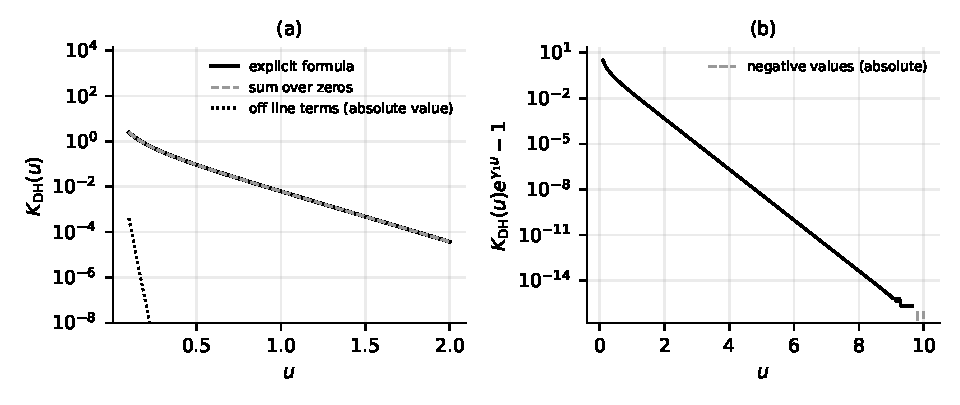
\includegraphics[width=\textwidth]{fig/bsy_dhlevy.pdf}
\caption{The Davenport and Heilbronn L\'evy density. Left: $K_{\mathrm{DH}}$ by the explicit formula and by the sum over zeros, with the off line terms in absolute value. Right: $K_{\mathrm{DH}}(u)e^{\gamma_1u}-1$ on a logarithmic scale; the quantity $K_{\mathrm{DH}}(u)e^{\gamma_1u}$ tends to $1$, from above for large $u$ since the first zero is simple and the second lies on the line. Beyond $u=9$ the right panel shows rounding noise.}\label{bsy:fig:dhlevy}
\end{figure}

Positivity of the trace is not automatic for Dirichlet series with a functional equation, as the following remark shows.

\begin{remark}[a negative trace]\label{bsy:rem:negW}
{\emergencystretch=8em Let $B(s)=L(s,\chi_4)$, $\Lambda_B(s)=(4/\pi)^{s/2}\Gamma(\frac{s+1}2)B(s)$, let $p<q<2p$ be odd primes, and put $a=\frac12\log(pq)$, $b=\frac12\log(p/q)$ and $P(s)=1+2\sqrt p\,p^{-s}+2\sqrt q\,q^{-s}+\sqrt{pq}\,(pq)^{-s}$. Then
\[
\Bigl(\frac{4pq}\pi\Bigr)^{s/2}\Gamma\Bigl(\frac{s+1}2\Bigr)P(s)B(s)=2(pq)^{1/4}\Lambda_B(s)\bigl[\cosh(a(s-\tfrac12))+2\cosh(b(s-\tfrac12))\bigr],
\]}
which is entire of order one, real and positive on $\mathbb R$, and invariant under $s\mapsto1-s$. With $B_p=B\,(1-\chi_4(p)p^{-s})$, the $L$ function of the character modulo $4p$ induced by $\chi_4$, $p^{-s}B=\chi_4(p)(B-B_p)$, and similarly for $q$ and $pq$, so $PB$ is a real linear combination of $L$ functions of characters modulo $4$, $4p$, $4q$ and $4pq$. With $z=a(s-\frac12)$ and $\epsilon=b/a$, at a zero of $H_\epsilon(z)=\cosh z+2\cosh(\epsilon z)$ we have $|\sinh x|\le2\cosh(x/2)$, so $|x|<3$; by Rouch\'e's theorem against $\cosh z+2$, for $|\epsilon|$ small $H_\epsilon$ has exactly two zeros with $0\le\Im z\le2\pi$, near $\pm\operatorname{arcosh}2+i\pi$. For $p$ large they give the lowest zeros of the completed function above the real axis, a pair $\frac12\pm\delta_0+i\gamma_0$ with $\delta_0>0$ and $\gamma_0$ below the first zero of $\Lambda_B$; hence the trace satisfies $K(u)=2e^{-\gamma_0u}\cos(\delta_0u)+O(e^{-(\gamma_0+\eta)u})$ for some $\eta>0$, and $K((2k+1)\pi/\delta_0)<0$ for all large $k$. So the reciprocal of this completed function is not infinitely divisible. For $p=101$, $q=103$: $\delta_0=0.28475$, $\gamma_0=0.67928$ and $K(\pi/\delta_0)=-1.11\times10^{-3}$ (computed in floating point from the zeros of $H_\epsilon$ with $m\le5$ and the first five zeros of $L(s,\chi_4)$).
\end{remark}

\noindent The primitive version of the question stays open (Open problem~\ref{bsy:op:dh}).

\section{Brownian motion and a probabilistic reading of the criterion}\label{bsy:sec:bm}

The Cauchy kernel $P_{1-\theta}(t_0-\cdot)$ is the law of the height at which planar Brownian motion $B$ started at $1+it_0$ first hits the line $\Re s=\theta$. As in Section~\ref{bp:sec:planar}, the Cauchy process is Brownian motion run along the first passage times of an independent Brownian motion, indexed by the level.

\begin{proposition}[the criterion as optional stopping]\label{bsy:prop:yor}
Let $B$ be a planar Brownian motion started at $s_0=1+it_0$, $\tau$ its hitting time of the line $\{\Re s=\theta\}$ and $H=\{\Re s>\theta\}$. Then $\log|h_\theta(B_\tau)|$ is integrable and
\[
\E\bigl[\log|h_\theta(B_\tau)|\bigr]=\log|h_\theta(s_0)|+\sum_{\beta>\theta}G_\theta(s_0,\rho).
\]
The process $\log|h_\theta(B_{t\wedge\tau})|$ is a local martingale and a submartingale; it is a uniformly integrable martingale if and only if $\zeta$ has no zero with $\beta>\theta$. Each zero contributes its Riesz mass $2\pi$, times $\frac12$, times the value at $\rho$ of $\pi^{-1}G_\theta(s_0,\cdot)$, the density of the expected occupation measure of $B$ killed at $\tau$. Planar Brownian motion almost surely never visits a given point, so no local time at the zeros is involved.
\end{proposition}

\begin{proof}
The law of $B_\tau$ is $P_{1-\theta}(t_0-\tau)\,d\tau$ on the line (Section~\ref{bp:sec:planar}) and $|h_\theta|=|\zeta|$ there, so integrability and the identity are Theorem~\ref{bsy:thm:bsy}. The function $\log|h_\theta|$ is harmonic on $H$ off the zeros, which $B$ almost surely never visits; stopping at the exit times of the compact sets $\{|s|\le n,\ \Re s\ge\theta+\frac1n,\ |s-\rho|\ge\frac1n\ \text{for all}\ \rho\}$ shows that $\log|h_\theta(B_{t\wedge\tau})|$ is a local martingale. By \eqref{bsy:eq:nevanlinna}, $\log|h_\theta|=v-\sum_{\beta>\theta}G_\theta(\cdot,\rho)$ on $H$, where $v(z)=\E_z\log|\zeta(B_\tau)|$; by the strong Markov property $v(B_{t\wedge\tau})=\E[\log|\zeta(B_\tau)|\mid\mathcal F_{t\wedge\tau}]$ is a uniformly integrable martingale. Each $G_\theta(B_{t\wedge\tau},\rho)$ is a positive local martingale, hence a supermartingale, and so is their sum, by monotone convergence and $\sum G_\theta(s_0,\rho)<\infty$. So $\log|h_\theta(B_{t\wedge\tau})|$ is a submartingale. If there is a zero with $\beta>\theta$, its terminal value has expectation strictly above its initial value, so it is not a uniformly integrable martingale; if there is none it equals $v(B_{t\wedge\tau})$. Finally $\pi^{-1}G_\theta(\cdot,z)$ is the Green function of $H$ for the generator $\frac12\Delta$, since $\frac12\Delta\,\pi^{-1}G_\theta(\cdot,z)=-\delta_z$ and $G_\theta(\cdot,z)=0$ on $\partial H$, which gives the occupation statement.
\end{proof}

So RH says that $\log|h_{1/2}|$, whose boundary values are $\log|\zeta|$, is a fair game for Brownian motion stopped on the critical line, and each zero off the line is a source of drift. Under RH, $m_\sigma(t)$ is the hitting density of the critical line for Brownian motion from $\sigma+it$, summed over the critical zeros, and a zero off the line is the one thing that can make that density negative.

\subsection{The complex logarithm: a conformal martingale}\label{bsy:sec:cmart}

Proposition~\ref{bsy:prop:yor} uses only the real part of $\log h_\theta$. Under the quasi Riemann hypothesis the whole complex logarithm is analytic on the half plane, and conformal invariance then fixes all the analytic moments of $\log h_\theta$ on the line under harmonic measure; with the energy identity below they give its second order structure.

\begin{theorem}[moments of $\log h_\theta$ under harmonic measure]\label{bsy:thm:cmart}
Assume $\mathrm{QRH}(\theta)$, $\frac12\le\theta<1$. Let $L$ be the analytic logarithm of $h_\theta$ on $H=\{\Re s>\theta\}$ with $L(\sigma+it)\to0$ as $\sigma\to+\infty$. For almost every $\tau$ the limit $Z(\tau)=X(\tau)+iY(\tau)=\lim_{\sigma\downarrow\theta}L(\sigma+i\tau)$ exists, $X(\tau)=\log|\zeta(\theta+i\tau)|$, and $Y(\tau)=\arg h_\theta(\theta+i\tau)$ continued along the horizontal path from $+\infty$. Let $\tau$ have law $P_{1-\theta}(t_0-\cdot)$ and $z_0=x_0+iy_0=L(1+it_0)$. Then $\E|Z|^p<\infty$ for every $p<\infty$, $\E[Z^k]=z_0^k$ for every $k\ge1$, and in particular $\E X=x_0$, $\E Y=y_0$, $\mathrm{Var}\,X=\mathrm{Var}\,Y$, $\mathrm{Cov}(X,Y)=0$, with
\[
\mathrm{Var}\,X=\mathrm{Var}\,Y=\frac1\pi\iint_{H}G_\theta(1+it_0,w)\,\Bigl|\frac{h_\theta'}{h_\theta}(w)\Bigr|^2\,dA(w).
\]
\end{theorem}

\begin{proof}
Under $\mathrm{QRH}(\theta)$, $h_\theta$ is analytic and zero free on $H$ ($h_\theta(1)=1/(2-2\theta)$), so $L$ exists. % UNCHECKED: Duren70, Theorem 4.1 as the statement of M. Riesz's theorem
By Theorem~\ref{bsy:thm:bsy} with an empty sum, $\Re L=\log|h_\theta|$ is the Poisson integral of $X$, and $X$ has every moment under $P_{1-\theta}(t_0-\cdot)$ by Lemma~\ref{bsy:lem:var}. The map $w=(s-1-it_0)/(s-2\theta+1-it_0)$ sends $H$ onto the unit disc, $1+it_0$ to $0$, and the harmonic measure to normalised arc length; put $F=L\circ s(w)$. Then $\Re F$ is the Poisson integral of a function in $L^p$ of the circle for every $p<\infty$, so by M.~Riesz's theorem on conjugate functions \cite[Theorem 4.1]{Duren70} $F\in H^p$ for every $p<\infty$. Hence $F$ has nontangential limits $F^*$ almost everywhere, with $F^*=Z$: at boundary points where $h_\theta\ne0$, $L$ is continuous up to the line and the horizontal convention gives the same value, and the boundary zeros form a null set. For $k\ge1$, $F^k\in H^1$, so $\E[Z^k]=\int(F^*)^k\frac{d\phi}{2\pi}=F(0)^k=z_0^k$. With $k=1,2$, $\E[(Z-z_0)^2]=0$, that is $\E(X-x_0)^2=\E(Y-y_0)^2$ and $\E(X-x_0)(Y-y_0)=0$. Finally, by the Littlewood and Paley identity, $\E|Z-z_0|^2=\|F-F(0)\|_{H^2}^2=\frac2\pi\iint_{\mathbb D}|F'(w)|^2\log\frac1{|w|}\,dA(w)$, and since $\log(1/|w(s)|)=G_\theta(1+it_0,s)$ and $|F'(w)|^2dA(w)=|L'(s)|^2dA(s)$, this is $\frac2\pi\iint_HG_\theta(1+it_0,s)|L'(s)|^2dA(s)$, half of it for each coordinate.
\end{proof}

\begin{remark}[the Brownian reading]
For planar Brownian motion $B$ from $1+it_0$, stopped at its hitting time $T$ of the line, $L(B_{t\wedge T})=z_0+W_{A_{t\wedge T}}$ with $A_t=\int_0^t|L'(B_r)|^2\,dr$ and a complex Brownian motion $W$ (L\'evy's theorem; the clock is adapted, not independent of $W$). The bound $|F|^p\le P[|F^*|^p]$ of the proof is the harmonic majorant that makes the stopped powers uniformly integrable, so $\E[Z^k]=z_0^k$ is optional stopping. A zero of multiplicity $q$ to the right of the line removes this argument and makes $Y$ jump upwards by $2\pi q$ at its height; a zero on the line itself gives a jump $\pi q$ already under $\mathrm{QRH}(\theta)$.
\end{remark}

The coordinate $Y$ is $\arg h_\theta$ continued along the horizontal path, not the raw argument of $\zeta$. The raw argument differs from it by an explicit term, of the order of $2\arctan\frac{1-\theta}t$, and the identities of the theorem fail for it: at $\theta=\frac12$, $t_0=0$ under RH the variance of $\arg\zeta$ exceeds that of $\log|\zeta|$ by more than $\pi^2/3$. Indeed, with $w=(s-1)/s$ the raw argument is $Y-\phi$, where $\phi=\operatorname{Arg}w(\frac12+i\tau)$ is uniform on $(-\pi,\pi)$, so $\mathrm{Var}\,\phi=\pi^2/3$. Writing $F(w)=\sum_{n\ge1}a_nw^n$ as in the proof of Theorem~\ref{bsy:thm:cmart} and using $\E[\phi\sin n\phi]=(-1)^{n+1}/n$ gives $\mathrm{Cov}(Y,\phi)=-\int_0^1F(-r)\,dr/r$, and $F(-r)=\log h_{1/2}(\frac1{1+r})>0$ because $h_{1/2}(s)=1+(1-s)\int_1^\infty\{x\}x^{-s-1}\,dx>1$ for $\frac12<s<1$. Hence $\mathrm{Var}(Y-\phi)=\mathrm{Var}\,X+\frac{\pi^2}3-2\,\mathrm{Cov}(Y,\phi)>\mathrm{Var}\,X+\frac{\pi^2}3$.

The moments do not determine the joint law of $(X,Y)$ by themselves; the law is the image of the Cauchy law under $L$. What the theorem adds is the moment identities and the variance formula. Selberg's central limit theorem says that for $t$ uniform on $[T,2T]$, $\log|\zeta(\frac12+it)|$ and $\arg\zeta(\frac12+it)$ are asymptotically independent normals with the same variance $\frac12\log\log T$. Theorem~\ref{bsy:thm:cmart} is an exact finite height counterpart: under $\mathrm{QRH}(\theta)$, at every height, the two coordinates have equal variances and zero covariance under harmonic measure. A zero to the right of the line removes this proof: the logarithm then has a branch point in the half plane, and $Y$ jumps by $2\pi q$ at the height of a zero of multiplicity $q$.

\begin{table}[h]
\centering\scriptsize\setlength{\tabcolsep}{3pt}
\begin{tabular}{lccccccc}
\toprule
 & $\theta$ & $t_0$ & $\E X-x_0$ & $\E Y-y_0$ & $\mathrm{Var}\,X$ & $\mathrm{Var}\,Y$ & $\mathrm{Cov}(X,Y)$\\
\midrule
$\zeta$ & $\tfrac12$ & 0 & $0.0000$ & $0.0000$ & $0.1415$ & $0.1415$ & $0.0000$\\
$\zeta$ & $\tfrac12$ & 85.7 & $0.0000$ & $0.0000$ & $0.7056$ & $0.7056$ & $0.0000$\\
$\zeta$ & $\tfrac12$ & 1000 & $0.0000$ & $0.0000$ & $1.0539$ & $1.0539$ & $0.0000$\\
$\zeta$ & $\tfrac12$ & 5000 & $0.0000$ & $0.0000$ & $1.1298$ & $1.1298$ & $0.0000$\\
$\zeta$ & $\tfrac34$ & 85.7 & $0.0000$ & $0.0000$ & $0.1341$ & $0.1341$ & $0.0000$\\
DH & $\tfrac12$ & 85.7 & $+1.4407$ & $-0.0016$ & $0.6410$ & $4.4414$ & $-0.0727$\\
DH & $\tfrac34$ & 85.7 & $+0.4770$ & $-0.0003$ & $1.0124$ & $3.2682$ & $-0.0162$\\
\bottomrule
\end{tabular}
\caption{Moments of $Z=\log h_\theta(\theta+i\tau)$ under $P_{1-\theta}(t_0-\cdot)$, computed in floating point (\texttt{code/bsy\_cm.py}, shared evaluator \texttt{code/bsy\_zdh.py}): Poisson weighted panels between the zeros with tanh sinh nodes, midpoint cells beyond distance $1000$ out to $|\tau-t_0|\le13000$, and the mass beyond the window ($2.45\times10^{-5}$ at $\theta=\frac12$, $1.22\times10^{-5}$ at $\theta=\frac34$) estimated from the sample moments of the outer window. Entries are from the finer of two meshes; the larger of the difference between the meshes and half the tail correction is at most $2.1\times10^{-5}$ in every entry (the row at height $5000$ is in \texttt{data/bsy\_cm\_5000.json}). For $\zeta$ the equal variance and zero covariance identities of Theorem~\ref{bsy:thm:cmart} hold to that accuracy; for Davenport and Heilbronn (DH), with $h=f$, they fail at both levels.}\label{bsy:tab:cm}
\end{table}

Table~\ref{bsy:tab:cm} tests Theorem~\ref{bsy:thm:cmart}. For $\zeta$ the variances of $\log|\zeta|$ and $\arg h_\theta$ agree and the covariance vanishes to $2.1\times10^{-5}$ in every row, the size of the differences between the two meshes. For Davenport and Heilbronn the variance of the argument is $6.9$ times that of the modulus at $\theta=\frac12$ and $3.2$ times at $\theta=\frac34$, as the jump of $Y$ at the height of the zero suggests (an observation, not a consequence of the jump), and the first moment shows the defect of Theorem~\ref{bsy:thm:bsy}. At the three positive heights shown the variance at $\theta=\frac12$ is close to $\frac12\log\log t_0$ ($0.71$ against $0.75$ at height $85.7$, $1.05$ against $0.97$ at height $1000$, $1.13$ against $1.07$ at height $5000$), the scale of Selberg's theorem, which concerns $t$ uniform on $[T,2T]$ and implies nothing for a window of fixed width at a given centre.

\subsection{The defect of the complex moments}\label{bsy:sec:cuts}

Without $\mathrm{QRH}(\theta)$ the moments of $Z$ have explicit defects. The contour argument of Bui, Lester and Milinovich \cite{BLM14} moves the line of integration across horizontal cuts from the zeros for the logarithm itself; the extension to every polynomial moment is proved here.

\begin{proposition}[complex moments through the cuts]\label{bsy:prop:cuts}
Let $\frac12\le\theta<1$, $z=1+it_0$, $z^*=2\theta-1+it_0$ and $K(s)=\frac1{s-z^*}-\frac1{s-z}$. For each ordinate $\gamma$ of a zero with $\beta>\theta$ let $b_\gamma$ be the largest real part of the zeros with that ordinate, $C_\gamma=[\theta+i\gamma,\,b_\gamma+i\gamma]$, and for $x+i\gamma\in C_\gamma$ let $M_\gamma(x)$ be the number of zeros $\beta'+i\gamma$ with $\beta'>x$, counted with multiplicity. Let $L$ be the logarithm of $h_\theta$ on $\{\Re s>\theta\}$ minus the cuts, continued along horizontal paths from $+\infty$, where it tends to $0$; let $z_0=L(z)$ and let $L_-$ be the boundary value from below on $C_\gamma$, so that the value above minus the value below is $2\pi iM_\gamma$. Let $Z(\tau)=\lim_{\sigma\downarrow\theta}L(\sigma+i\tau)$, which exists for almost every $\tau$, and $\tau\sim P_{1-\theta}(t_0-\cdot)$. Then for every polynomial $F$
\[
\E F(Z)-F(z_0)=\sum_\gamma\frac1{2\pi i}\int_{C_\gamma}\bigl[F(L_-+2\pi iM_\gamma)-F(L_-)\bigr]K(s)\,ds,
\]
each integral taken from left to right and the sum absolutely convergent. In particular
\[
D:=\E Z-z_0=\sum_{\beta>\theta}\Bigl[\log\frac{\rho-z^*}{\rho-z}-\log\frac{\theta+i\gamma-z^*}{\theta+i\gamma-z}\Bigr],
\]
the sum over the zeros with multiplicity and the logarithms continued along the cut, and
\[
\E Z^2-z_0^2=2\sum_\gamma\int_{C_\gamma}M_\gamma\,(L_-+\pi iM_\gamma)\,K(s)\,ds .
\]
The real part of the formula for $D$ is Theorem~\ref{bsy:thm:bsy} at $1+it_0$. The second order balance $\mathrm{Var}\,X=\mathrm{Var}\,Y$, $\mathrm{Cov}(X,Y)=0$ holds exactly when $2\sum_\gamma\int_{C_\gamma}M_\gamma\,(L_-+\pi iM_\gamma-z_0)\,K\,ds=D^2$. When the zeros with $\beta>\theta$ are simple with distinct ordinates, $M_\gamma=1$ on every cut and $L_-+\pi i$ is the mean of the two boundary values.
\end{proposition}

\begin{proof}
On the line $K(\theta+i\tau)=2a/(a^2+(\tau-t_0)^2)$ with $a=1-\theta$, so $K(s)\,ds/(2\pi i)=P_{1-\theta}(t_0-\tau)\,d\tau$ there and $\E F(Z)=\frac1{2\pi i}\int F(L)K\,ds$ along the line upwards. Take the rectangle $\theta\le\Re s\le X$, $|\Im s-t_0|\le T$, with $t_0\pm T$ not ordinates of zeros; remove thin strips along the cuts, small discs about their right ends and about the zeros on them, and small half discs about the zeros on the line, and apply the residue theorem to $F(L)K$ on the rest. Its only pole there is $z$, with residue $-F(z_0)$. With the positive orientation the line is traversed downwards and the upper bank of each cut from left to right, so, as the strips, discs and half discs shrink, $\frac1{2\pi i}\int F(L)K\,ds$ along the line upwards equals $F(z_0)$ plus the cut terms of the statement plus $\frac1{2\pi i}$ times the integrals over the other three sides; the discs and half discs contribute $O(r(1+|\log r|)^{\deg F})\to0$. In a fixed vertical strip $L(s)=A(s)+\sum m_\rho\log(s-\rho)$, the sum over the $O(\log(|t|+2))$ zeros with $|\gamma-t|\le1$, where $A=O(\log(|t|+2))$ (remove these factors in a disc and apply the Borel and Carath\'eodory lemma to the rest); so the integrals of $|L|^p$ over horizontal segments and over vertical segments of unit length are $O_p(\log^{c_p}(|t|+2))$. As $K=O(t^{-2})$ in the strip, the horizontal sides contribute $o(1)$ as $T\to\infty$, and the sum over the cuts converges absolutely, since there are $O(T\log T)$ zeros up to height $T$ and every cut is shorter than $\frac12$. On the right side $L(s)=O(2^{-\Re s})+O(|s|^{-1})$, which contributes $o(1)$ as $X\to\infty$. For $F(w)=w$ the jump is $2\pi iM_\gamma$, and $\int_{C_\gamma}M_\gamma K\,ds$ is the sum over the zeros with ordinate $\gamma$ of $\int_{\theta+i\gamma}^{\rho}K\,ds$; for $F(w)=w^2$ the jump is $4\pi iM_\gamma(L_-+\pi iM_\gamma)$. Finally $\E Z^2-(\E Z)^2=(\E Z^2-z_0^2)-2z_0D-D^2$.
\end{proof}

The same holds for the Davenport and Heilbronn function with $h=f$, provided no zero has $\gamma=t_0$ and $\beta\ge1$, so that $z$ lies off the cuts and $f(z)\ne0$; the proof uses the local factorisation and the Dirichlet series bounds of $f$ in place of those of $\zeta$.

We checked Proposition~\ref{bsy:prop:cuts} on the Davenport and Heilbronn function at $t_0=85.7$, with the zeros with $\beta>\theta$ below height $700$ and their conjugates (computed, floating point; \texttt{code/bsy\_cuts.py}, \texttt{data/bsy\_cuts.json}): $L$ is continued along each cut, the cut integrals use Gauss and Legendre nodes, and the jump across every cut is $2\pi i$ to $7$ digits. At $\theta=\frac12$ the cut formula gives $\E Z-z_0=1.4407-0.0016\,i$ and the balance defect $\mathrm{Var}\,X-\mathrm{Var}\,Y+2i\,\mathrm{Cov}(X,Y)=-3.8003-0.1455\,i$, against $1.4407-0.0016\,i$ and $-3.8004-0.1455\,i$ from the unrounded entries of Table~\ref{bsy:tab:cm}; at $\theta=\frac34$ it gives $0.4770-0.0003\,i$ and $-2.2558-0.0323\,i$, against $0.4770-0.0003\,i$ and $-2.2558-0.0323\,i$.

For one simple zero with $\beta>\theta$ the balance condition reads exactly $\bar L-z_0=\frac12D$ when $D\ne0$, where $\bar L=D^{-1}\int_C(L_-+\pi i)K\,ds$ is a mean of $L_-+\pi i$ along its cut with the complex weight $K/D$. For a zero far from $t_0$ the weight is nearly constant along the short cut, so $\bar L$ nearly does not depend on $t_0$, while $D\to0$; balance at every such $t_0$ would make $z_0=\log h_\theta(1+it_0)$ nearly constant, which it is not. This suggests that the balance fails for most $t_0$ when a zero lies to the right of the line (heuristic: the variation of $\bar L$ with $t_0$ has not been bounded). With several cuts the contributions can cancel, and no proof is known (Open problem~\ref{bsy:op:cmart}).
